\documentclass[12pt,letterpaper]{report}
\usepackage[margin=1in]{geometry}
\usepackage{graphicx}
\usepackage{amsmath}
\usepackage[font=small,labelfont=bf]{caption}
\usepackage[justification=centering]{caption}
\usepackage{tikz}
\usepackage{circuitikz}
\usepackage{siunitx}
\newlength \figwidth
\setlength \figwidth {0.75\linewidth}

\begin{document}

\title{E153 Laboratory Assignment \#3}
\author{Courtney Keeler and Stephen Pinto\\
Harvey Mudd College}
\date{October 21, 2013}
\maketitle

\section*{List of Materials}
\begin{itemize}
	\item Elenco LCM-1950 Multimeter
	\item 1N4001 diode
	\item standard value resistors
\end{itemize}

\section*{Purpose}
The purpose of this lab is to understand diodes and build circuits to measure the current through  a forward biased 1N4001 diode over ten orders of magnitude.

\section*{Procedure}

\begin{enumerate}
\item Construct the circuit shown in Figure \ref{fig:circuit_1}, where the 1 M$\Omega$ resistor represents the internal resistance of the digital multimeter.
\item Vary the value of V1 based on the values in Table %\ref{table:voltage_values}.
\item Use the voltage measured through the multimeter to calculate the voltage drop across the diode as well as the current through the diode.
\item Construct the circuit shown in Figure \ref{fig:circuit_2}, where the 1 M$\Omega$ resistor represents the internal resistance of the multimeter measuring the voltage drop across R2.
\item Vary the voltage V1 based on the values in Table %\ref{table:voltage_values}.
\item Use the measured voltage drop to calculate the current through the diode and the voltage drop across the diode.
\item Construct the circuit shown in Figure \ref{fig:circuit_3}, where two multimeters are used: one as an ammeter, and another as a voltmeter (as represented by the 1 M$\Omega$ resistor).
\item Vary the voltage of V1 based on the values in Table %\ref{table:voltage_values}.
\item Record the measured voltage drop across the diode and current running from the back of the diode to ground.
\end{enumerate}

\begin{figure}
\centering
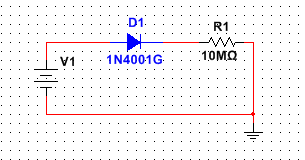
\includegraphics[width=\figwidth, keepaspectratio=true]{lab3/lab3_image_1.png}
\caption{Circuit to measure mid-range current values through the diode.}
\label{fig:circuit_1}
\end{figure}

\begin{figure}
\centering
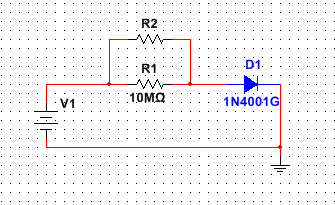
\includegraphics[width=\figwidth, keepaspectratio=true]{lab3/lab3_image_2.png}
\caption{Circuit to measure high-range current values through the diode. R2 = .969 k$\Omega$}
\label{fig:circuit_2}
\end{figure}

\begin{figure}
\centering
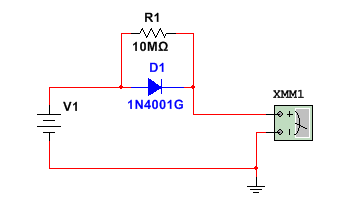
\includegraphics[width=\figwidth, keepaspectratio=true]{lab3/lab3_image_3.png}
\caption{Circuit to measure low-range current values through the diode.}
\label{fig:circuit_3}
\end{figure}

\section*{Results}

\section*{Analysis}

\section*{Calculations}

For the case of the circuit shown in Figure \ref{fig:circuit_1}, the voltage drop across a known resistance value is measured. Using Ohm's law, we can calculate
$$
I = \frac{V}{R}.
$$
Since the diode is in series with the resistor, and these are the only circuit elements, we know the current through the diode must be equal to the current through the resistor. 
We use KVL to calculate the voltage drop across the diode. We know the value of V1, the voltage into the circuit, and we know the voltage drop across the resistor. By KCL:
$$
V_{\text{in}} - V_{\text{drop across diode}} - V_{\text{drop across resistor}} = 0.
$$

For the case of the circuit shown in Figure \ref{fig:circuit_2}, the current going into the diode is the sum of the current through the multimeter (R1) and the 1 k$\Omega$ resistor (R2). Since V1 is known and the voltage drop across R2 is measured, we can calculate
$$
I_1 = \frac{V_{\text{measured drop}}}{R1}
$$
$$
I_2 = \frac{V_{\text{measured drop}}}{R2}
$$
We again use KVL to calculate the voltage drop across the diode:
$$
V_{\text{in}} - V_{\text{drop across R2}} - V_{\text{drop across diode}} = 0.
$$

\end{document}
